\vspace{-.5em}
\section{Our Proposal}
\vspace{-.5em}
In this paper, we aim at scaling logging and recovery process on multi-core machines, diluting the negative impact introduced by logging to transaction processing, and reducing fail-over time in presence of failures. To fulfill this goal, we propose a holistic approach to address the problems identified in the previous section, which consists of the following three techniques:

\noindent{\bf 1. Relaxing ordering constraints between log entries.} To avoid imposing unnecessary ordering, we maintain a partial order among entries, where the dependency between two entries implies that reordering them will violate application specific invariants. 

\noindent{\bf 2. Changing the logging granularity from page level to command level.} The benefit of logging commands is two-fold: (a) it significantly reduces the amount of data that needs to be flushed and consequently mitigates the overall I/O impacts; (b) commands contain rich application semantics, based on which we can explore operation commutativity to reduce false dependencies.

\noindent{\bf 3. Optimizing the log entry placement.} When distributing entries to a set of logs, we have to reduce cross-log dependencies and balance the log load as possible. 

We translate the above design rationale into the following {\bf System design.} First, we maintain a set of $N$ logs, where $N$ is equal to the total number of cores on a machine and each core is responsible for a dedicated log. We decouple the transaction processing and logging phases by maintaining two thread pools, namely an executor and flusher pool, whose size is also $N$. Our design has a log dispatcher that efficiently manages interactions between executors and flushers. Each executor processes database queries comprising a transaction, keeps log entries in its private buffer, and delivers content in its buffer to the log dispatcher upon commit. The log dispatcher collects log entries from different executors, performs a quick analysis to determine their dependencies and the best placement strategies, and distributes log entries to flushers. Finally, each flusher persists log entries to non-volatile storage and sends back an ``ACK'' to the corresponding executor to successfully complete a transaction.
When recovering, we launch $N$ workers and a coordinator, where each worker processes a log file to apply changes to database as independently as possible while communicating with coordinator to proceed when cross-log synchronization is needed.
\if 0
In this section, we will propose two new techniques to eliminate the cross-log dependencies, which will accelerate the logging and recovery.
\subsection{Vector Clock vs Lamport's Clock}
The order is defined in [] by Lamport's clock, which is a global total order and will incur unnecessary false dependeicies. For example, the right side of Fig.~\ref{fig:vectorclock} shows the Lamport's Clock in distributed Log, each block indicates one log entry. When H wants to commit, all of the changes before it must be flushed to disk even though some of them are indenpendent with each other, this kind of dependency is called false dependency and will incur performance slow down.

We can adopt Vector Clock to avoid the false dependency, whose order is partial, the left side of Fig.~\ref{fig:vectorclock} illustrates the Vector Clock in distributed Log. When H wants to commit, only the really dependent log entries are flush to disk, so we can flush part of the Logs rather than almost all of them.
\begin{figure}[htbp]
  \centering
  % Requires \usepackage{graphicx}
  %\vspace{-5pt}
  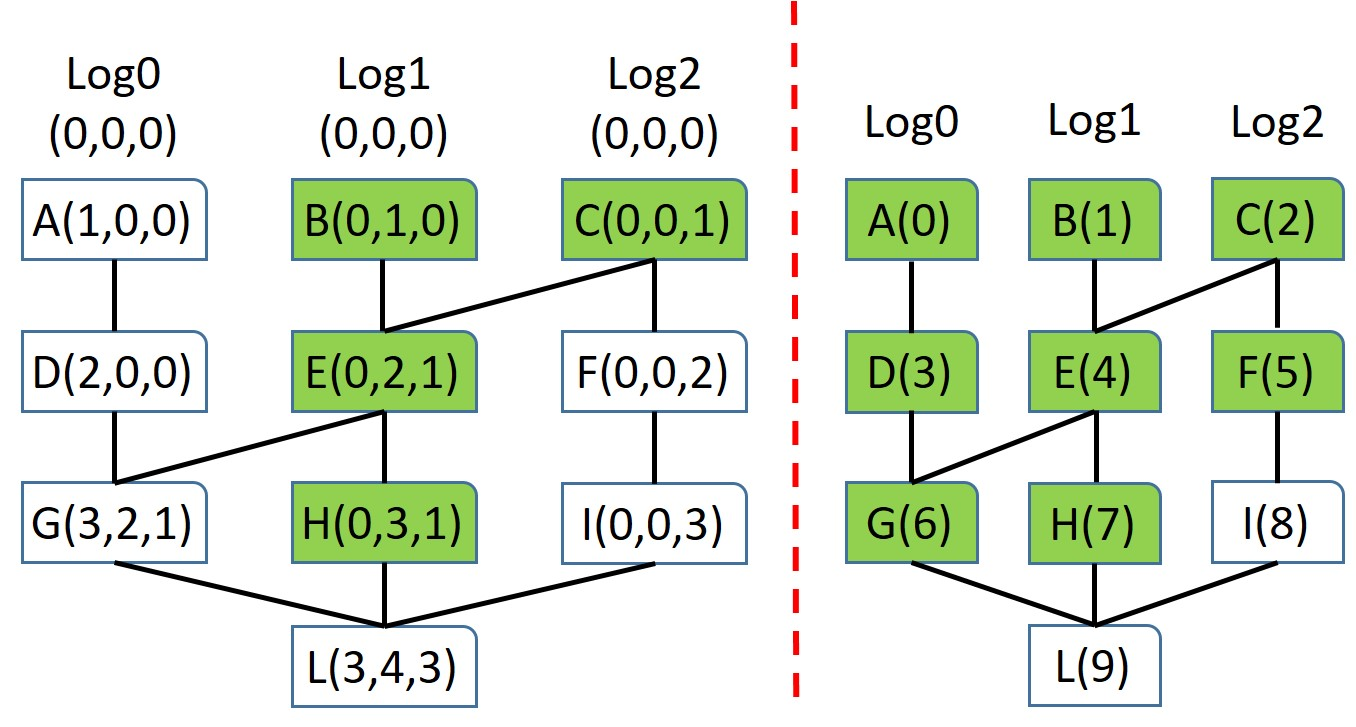
\includegraphics[width=1\linewidth]{vectorclock.jpg}\\
  %\vspace{-10pt}
  \caption{Vector Clock vs Lamport's Clock.}\label{fig:vectorclock}
   %\vspace{-10pt}
\end{figure}

\subsection{Conflict-free Replicated Data Types}
We can make some conflict operations commutative by using Conflict-free Replicated Data Types(CRDTs), which means that the result will be consistent even though commute the order of related operations. We give a simple example to propose our method. In the left side of Fig.~\ref{fig:crdt}, transaction 2(txn2) and 4(txn4) want to modify the same object A, and txn2 operates \texttt{A = A * 2}, then txn4 operates \texttt{A = A + 4}, the final result of A is 10. But if we commute the operations of txn2 and txn4, the result will be 14 and inconsistent. 

If we transfer the multiplication into addition such as the example in Fig.~\ref{fig:crdt} right side, the operation \texttt{A = A * 2} can be transferred as \texttt{A = A + 3}, we can issue operations of txn2 and txn4 without order to improve performance and the result will be always consistent.
\begin{figure}[htbp]
  \centering
  % Requires \usepackage{graphicx}
  %\vspace{-5pt}
  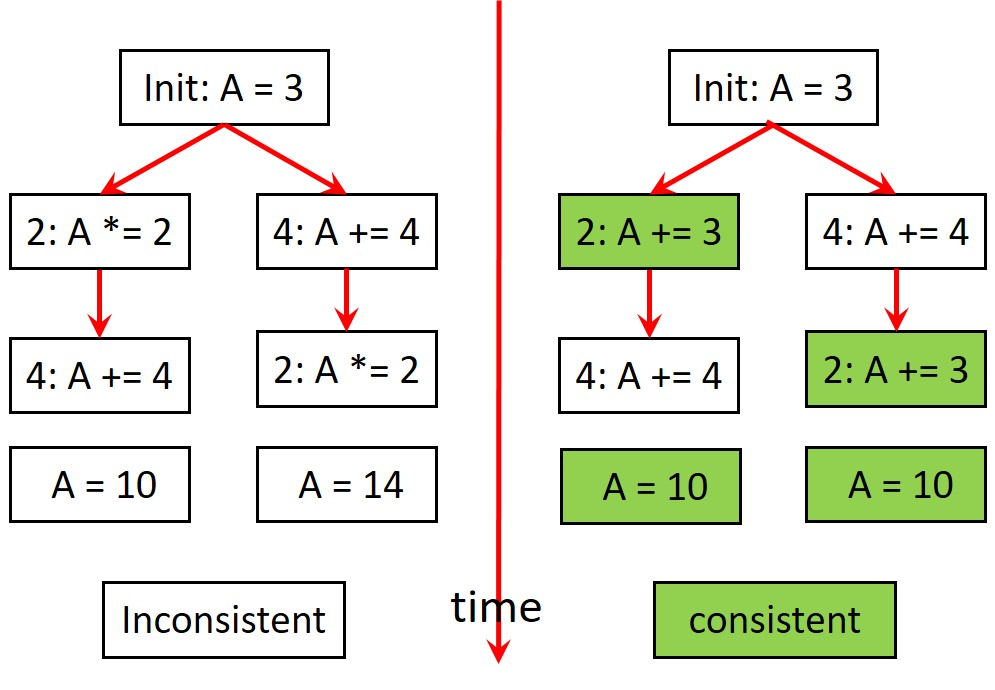
\includegraphics[width=1\linewidth]{CRDT.jpg}\\
  %\vspace{-10pt}
  \caption{Correlations update.}\label{fig:crdt}
   %\vspace{-10pt}
\end{figure}
\fi
% \begin{itemize} 圆点
%   \item \textbf{Set} 粗体 Clients could set data and access correlations to a specific file with this interface. New score will be embedded into system.
%   \item \textbf{Remove} Remove a specific correlation item from a file.
% \end{itemize}
% \textbf{Challenge 1} When there is overwritten to a file, as Fig.~\ref{fig:overwrite} shows, the new data is easy to make a analysis to find correlated files. But the overlayed data maybe contain links to related files, which are obsolete and should be removed simultaneously. However the covered data isn't in cache, so how to update the correlations is a challenge. We introduce a lazy update method. When a files overwrites, we make a \texttt{overwritten} tag on the file. Once the tagged file is accessed, system will make a semantic analysis again to rebuild correlations to keep consistency.
